\chapter{User Documentation}

\section{Display a Raster Map}

This tutorial describes how to get a raster tile map with OSM Vector
Tiles as data source.

\subsection{Result}

You get a basic raster tile map similar to the map below.

\hypertarget{osm-bright-map}{}

\subsection{Preparation}

\begin{enumerate}
\item
  \href{http://osm2vectortiles.org/data/download.html}{Download} an
  extract you want to serve.
\item
  \href{https://github.com/mapbox/mapbox-studio-osm-bright.tm2.git}{Download}
  the visual style.
\item
  Add both to the same directory and make sure that the have the same
  name
\end{enumerate}

\subsection{Install Kitematic}

\begin{enumerate}
\item
  \href{https://www.docker.com/docker-toolbox}{Download} and install
  Kitematic.
\item
  Start a new container by searching for \texttt{osm2vectortiles} and
  click create on the container called \texttt{serve}.
\end{enumerate}

\begin{figure}[H]
\centering
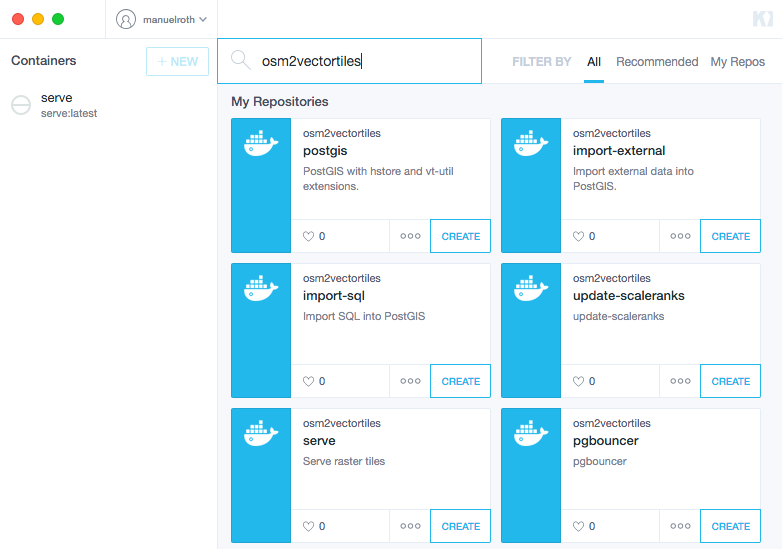
\includegraphics[width=1\textwidth]{images/search_container.png}
\caption{Search Container}
\end{figure}

\subsection{Kitematic Usage}\label{kitematic-usage}

When you start the container, it will complain about missing
\texttt{tm2} style projects.

\begin{figure}[H]
\centering
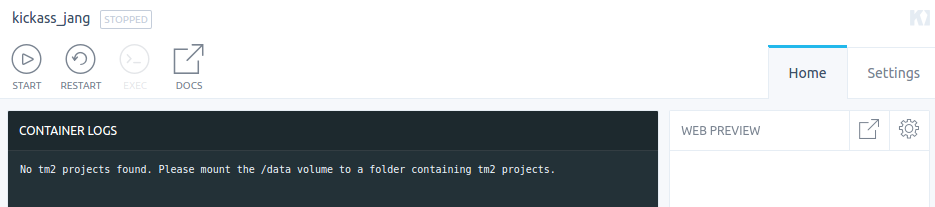
\includegraphics[width=1\textwidth]{images/tileserver_kitematic_started.png}
\caption{Container started unsucessfully}
\end{figure}

Mount your the directory containing the \texttt{mbtiles} files and
\texttt{tm2} style projects into the \texttt{/data} volume.

\begin{figure}[H]
\centering
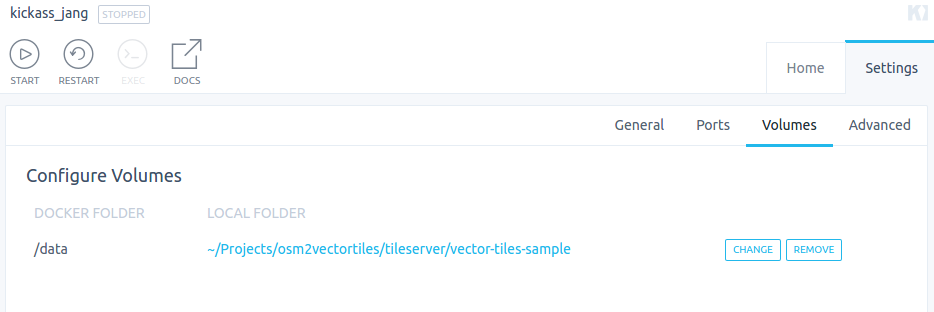
\includegraphics[width=1\textwidth]{images/tileserver_kitematic_volumes_configured.png}
\caption{Configured volumes for container}
\end{figure}

Now restart the container. You should be up and running serving
generated raster tiles.

\begin{figure}[H]
\centering
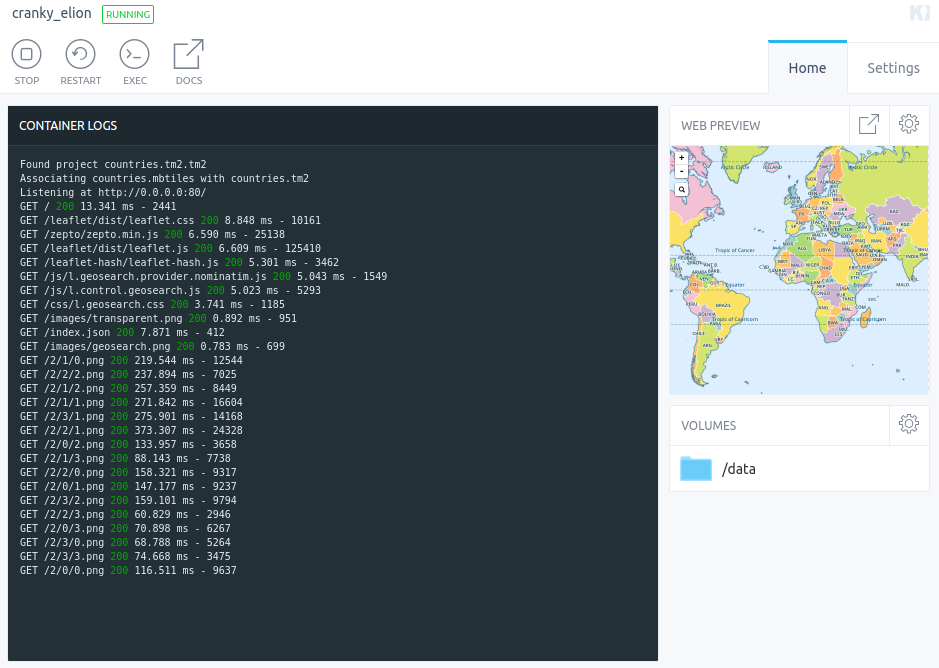
\includegraphics[width=1\textwidth]{images/tileserver_kitematic_running.png}
\caption{Container running and serving tiles}
\end{figure}

%-------------------------------
\section{Display Map with MapboxGL}\label{display-map-with-mapboxgl}

To display a custom MapboxGL based map you need to create a HTML file
and reference the public vector tile server of osm2vectortiles. You are
free to download and host the vector tiles yourself but we provide a
fast and distributed CDN service for serving the PBFs for you.

The easiest way to get started is using the
\texttt{mapbox-gl-js-exmaple} repository. Clone the repository and
change into the directory.

\begin{bashcode}
git clone https://github.com/osm2vectortiles/mapbox-gl-js-example.git
\end{bashcode}

\subsection{Configure Source, Fonts and
Sprites}\label{configure-source-fonts-and-sprites}

In order for Mapbox GL JS to work you also need to provide the
\href{https://www.mapbox.com/mapbox-gl-style-spec/\#glyphs}{fonts} and
\href{https://www.mapbox.com/mapbox-gl-style-spec/\#sprite}{sprites}.
These resources are contained in the folder \texttt{assets}.

The \href{https://www.mapbox.com/mapbox-gl-style-spec/}{Mapbox GL Style
JSON} of OSM Bright is located at \texttt{bright-v8.json}. You can
create your own styles with Mapbox Studio.

If you want to serve the Mapbox GL Style JSON without Mapbox you need to
configure three URLs.

\begin{enumerate}
\item
  Change the \texttt{sources} URL to the free osm2vectortile serve or
  use your own server
\item
  Change the \texttt{sprite} URL to the location of your sprites
\item
  Change the \texttt{glyphs} URL to the location of your fonts
\end{enumerate}

\begin{javascriptcode}
"sources": {
    "mapbox": {
        "url": "http://vectortiles.osm2vectortiles.org/world.json",
        "type": "vector"
    }
},
"sprite": "/assets/sprite",
"glyphs": "/assets/font/{fontstack}/{range}.pbf"
\end{javascriptcode}

\subsection{Initialize the Map}\label{initialize-the-map}

In order to serve a MapboxGL based map you need a
\href{https://www.mapbox.com/mapbox-gl-style-spec/}{Mapbox GL style
JSON} created with \href{https://www.mapbox.com/mapbox-studio/}{Mapbox
Studio}. In this example we will serve the free OSM Bright style
\href{https://github.com/mapbox/mapbox-gl-styles}{provided by Mapbox}.

The HTML file defines a full screen map and the CSS and JavaScript files
required by Mapbox GL JS. The \texttt{bright-v8.json} style is loaded
from the local directory.

Because we use the local sprites and fonts we don't need a Mapbox API
key.

\begin{htmlcode}
<!DOCTYPE html>
<html>
<head>
    <meta charset='utf-8' />
    <title>MapBox GL JS with osm2vectortiles Example</title>
    <meta name='viewport' content='initial-scale=1,maximum-scale=1,user-scalable=no' />
    <script src='//api.tiles.mapbox.com/mapbox-gl-js/v0.10.0/mapbox-gl.js'></script>
    <link href='//api.tiles.mapbox.com/mapbox-gl-js/v0.10.0/mapbox-gl.css' rel='stylesheet' />
    <style>
        body { margin:0; padding:0; }
        #map { position:absolute; top:0; bottom:0; width:100%; }
    </style>
</head>
<body>

<div id='map'></div>
<script>
mapboxgl.accessToken = 'NOT-REQUIRED-WITH-YOUR-VECTOR-TILES-DATA';

var map = new mapboxgl.Map({
    container: 'map',
    style: '/bright-v8.json',
    center: [8.3221, 46.5928],
    zoom: 1,
    hash: true
});
map.addControl(new mapboxgl.Navigation());
</script>
</body>
</html>
\end{htmlcode}


\subsection{Serve the Map}

You need a simple HTTP server for serving the HTML and

%-------------------------------

%-------------------------------

\section{Create a new Style with Mapbox Studio
Classic}\label{create-a-new-style-with-mapbox-studio-classic}

You can use
\href{https://www.mapbox.com/help/getting-started-studio/}{the same
resources from Mapbox} for learning how to design maps with Mapbox
Studio Classic. This tutorial will show you how to customize the OSM
Bright style.

Download \href{https://www.mapbox.com/mapbox-studio-classic/}{Mapbox
Studo Classic} to create your first map.

\subsection{Create new style project}\label{create-new-style-project}

Create a new style project based of OSM Bright. You can also start with
a blank slate but it is easier to get started from an existing style.

In \texttt{Styles\ and\ Resources} create a new style and choose
\texttt{OSM\ Bright\ 2}. Then save your project.

\begin{figure}[H]
\centering
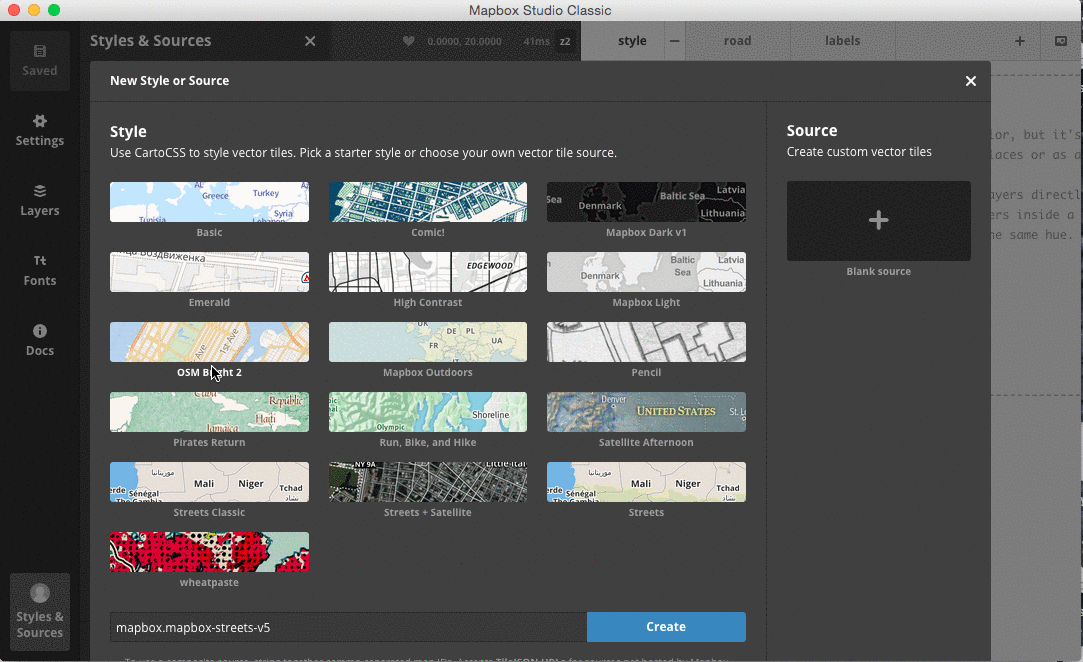
\includegraphics[width=1\textwidth]{images/mapbox_classic_create_project.png}
\caption{Create new project with Mapbox Studio Classic}
\end{figure}

\subsection{Switch to osm2vectortiles}\label{switch-to-osm2vectortiles}

Now you are based of the vector tiles from Mapbox Streets. To use our
free and Open Source vector tiles you need to \texttt{Change\ Source} in
\texttt{Layers}.

Enter the \href{https://github.com/mapbox/tilejson-spec}{TileJSON} url
of our vectortiles server
\texttt{vectortiles.osm2vectortiles.org/world.json}. You can later
replace this with your own vector tiles server if you want to serve
everything by yourself.

Because our vector tiles are to a large part Mapbox Streets compatible
you won't see any drastic changes. In fact you could even continue
styling your project with Mapbox Streets and make the switch at the
deployment stage of the project.

\begin{figure}[htbp]
\centering
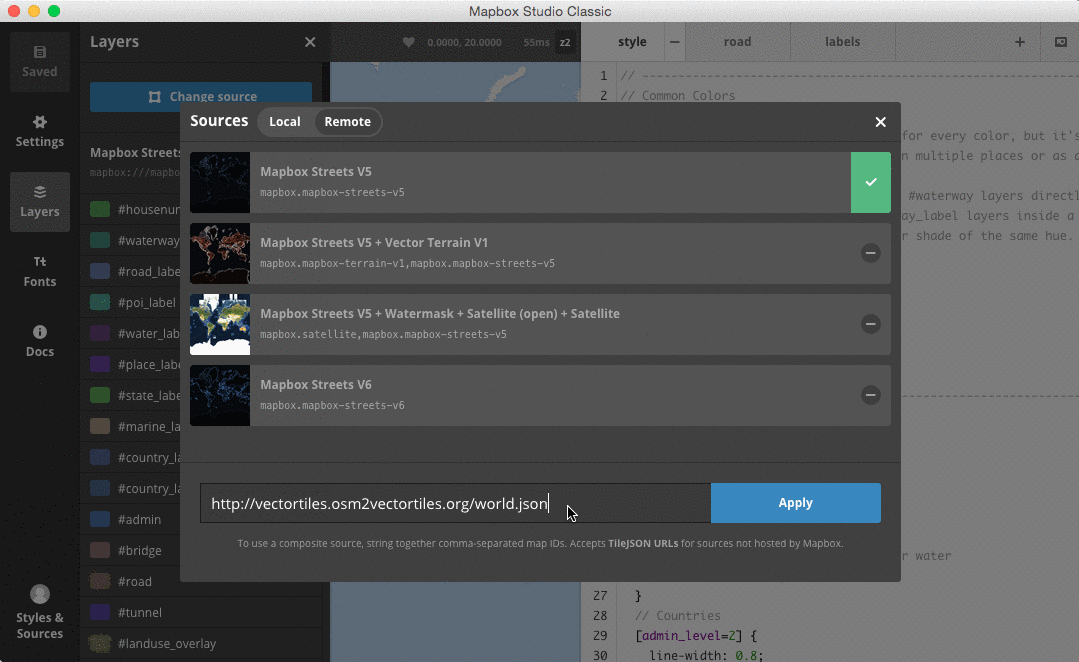
\includegraphics[width=1\textwidth]{images/mapbox_classic_switch_osm2vectortiles.png}
\caption{Switch to osm2vectortiles in Mapbox Studio Classic}
\end{figure}

\subsection{Deploy your Map}\label{deploy-your-map}

Because you are no longer bound to Mapbox for hosting you can now host
the maps yourself and save money.

%-------------------------------

\section{Create a new Style with new Mapbox
Studio}\label{create-a-new-style-with-new-mapbox-studio}

Mapbox Studio is the new Map design platform by Mapbox. Mapbox provides
\href{https://www.mapbox.com/help/getting-started-mapbox-studio-1/}{great
resources for getting started} how to design your own maps. This
tutorial will show you how to customize the OSM Bright style for Mapbox
GL.

Visit \href{https://www.mapbox.com/studio/}{the Mapbox Studio Editor}
and follow the tutorial.

\subsection{Create new style project}\label{create-new-style-project}

Create a new style project. Make sure you start of a base map that only
requires Mapbox Streets. A Mapbox Terrain equivalent is not available by
osm2vectortiles.

In \texttt{Styles} create a new style, choose \texttt{Bright} and save
your project.

\begin{figure}[H]
\centering
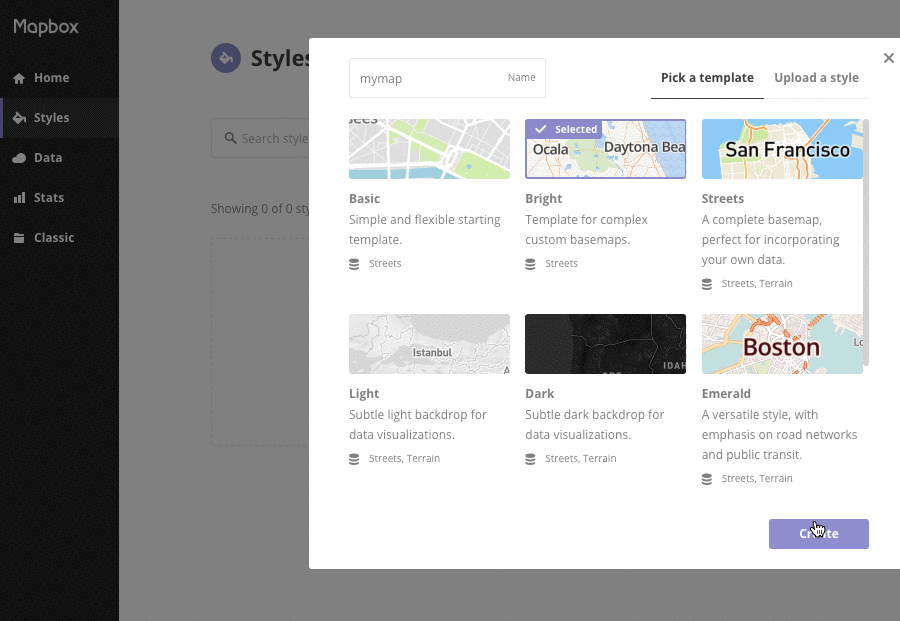
\includegraphics[width=1\textwidth]{images/mapbox_studio_create_style.png}
\caption{Create new project with new Mapbox Studio}
\end{figure}

\subsection{Switch to osm2vectortiles}\label{switch-to-osm2vectortiles}

In the new Mapbox Studio you can no longer specify a
\href{https://github.com/mapbox/tilejson-spec}{TileJSON} url of a custom
vectortiles server. Therefore it is best to work with the original
Mapbox Streets v6 data in the editor and make the switch to
osm2vectortiles at the deployment step. This works because our vector
tiles are to a large part Mapbox Streets v6 compatible.

Because users have an upload limit for their own data sources you cannot
upload the osm2vectortiles world file to Mapbox Studio and style it
directly. However if you want to work with the real data you can choose
an extract which is quite small (below 100MB) and upload it to Mapbox
Studio and work on this sample extract to create your map.

%--------------------------------------------------------------
\section{Serve Raster Tiles With Docker}

You can render raster tiles from a Mapbox Studio Classic \textbf{.tm2}
style project and a vector tiles file with the help of Docker and
\href{https://github.com/mojodna/tessera}{tessera}. For a single map you
can serve up to 50 users concurrently with a standard 4GB VPS server
with Docker installed.

\subsection{Preparation}\label{preparation}

\begin{enumerate}
\item
  Download MBTiles
\item
  Clone a visual style project
\item
  Add both to the same directory
\end{enumerate}

\subsubsection{Download MBTiles}\label{download-mbtiles}

On the server download your desired extract of a country or the entire
world MBTiles from http://osm2vectortiles.org/data/download.html.

\begin{bashcode}
wget -c https://osm2vectortiles-downloads.os.zhdk.cloud.switch.ch/v1.0/world.mbtiles
\end{bashcode}

\subsubsection{Clone the Style Project}\label{clone-the-style-project}

Clone your custom style project or in this example the official OSM
Bright style.

\begin{bashcode}
git clone https://github.com/mapbox/mapbox-studio-osm-bright.tm2.git
\end{bashcode}

\subsection{Run the raster tile
server}\label{run-the-raster-tile-server}

Make sure you have the style project and the MBTiles file in the same
directory.

Now run Docker via the command line to serve raster tiles. This will
serve the current directory at port 80. If your machine is accessible at
port 80 you can already see your map.

\begin{bashcode}
docker run -v \$(pwd):/data -p 80:80 osm2vectortiles/serve
\end{bashcode}

\subsection{Use the Map from Leaflet}\label{use-the-map-from-leaflet}

The server will now provide a TileJSON endpoint at the service url of
the map. For this example the TileJSON endpoint is
http://localhost/mapbox-studio-osm-bright/index.json. You can reference
this TileJSON endpoint in the leaflet configuration.

The HTML file will display a fullscreen Leaflet map using the raster
tiles from our raster tile server as a base layer. You can now add
additional layer on top of it or add interactivity.

\begin{htmlcode}
<!DOCTYPE html>
<html>
  <head>
    <meta charset=utf-8 />
    <title>A simple map</title>
    <meta name='viewport' content='initial-scale=1,maximum-scale=1,user-scalable=no' />
    <script src='https://api.mapbox.com/mapbox.js/v2.2.2/mapbox.js'></script>
    <link href='https://api.mapbox.com/mapbox.js/v2.2.2/mapbox.css' rel='stylesheet' />
    <style>
      body { margin:0; padding:0; }
      #map { position:absolute; top:0; bottom:0; width:100%; }
    </style>
  </head>
<body>
<div id='map'></div>
<script>
  var map = L.mapbox.map('map', 'mapbox.light', {
    minZoom: 8,
  }).setView([46.806, 8.091], 8);
  var overlay = L.mapbox.tileLayer('http://localhost/mapbox-studio-osm-bright/index.json').addTo(map);
</script>
</body>
</html>
\end{htmlcode}